% Opsætter KU Tex dokument
%%%%%%%%%%%%%%%%%%%%%%%%%%%%%%%%%%%%%%%%%%%%%%%%%%%%%%%%%%%%%%%%%%%%%%%%%%%%%%%%
\documentclass{article}                                                        %
\usepackage[a4paper, hmargin={2.8cm, 2.8cm}, vmargin={2.5cm, 2.5cm}]{geometry} %
\usepackage{eso-pic}  % \AddToShipoutPicture                                   %
\usepackage{graphicx} % \includegraphics                                       %
%\usepackage{subfig} - Can not be used with subcaption package (for subfigures)
\usepackage{setspace}                                                        %
%%%%%%%%%%%%%%%%%%%%%%%%%%%%%%%%%%%%%%%%%%%%%%%%%%%%%%%%%%%%%%%%%%%%%%%%%%%%%%%%

% Pakker til skrifttyper, tekst osv.
%%%%%%%%%%%%%%%%%%%%%%%%%%%%%%%%%%%%%%%%%%%%%%%%%%%%%%%%%%%%%%%%%%%%%%%%%%%%%%%%
    \usepackage[utf8]{inputenc}  % Implementere Unicode                        %
    \usepackage[T1]{fontenc}     % Unicode skrifttype fx. é skrives som 1 tegn %
    \usepackage[english]{babel}   % Dansk Ordbog                                %
    \usepackage{microtype}       % Forbedre linjeombrydningen                  %
    \usepackage{libertine}       % Skrifttype                                  %
%%%%%%%%%%%%%%%%%%%%%%%%%%%%%%%%%%%%%%%%%%%%%%%%%%%%%%%%%%%%%%%%%%%%%%%%%%%%%%%%

% Pakker til matematik og kode.
%%%%%%%%%%%%%%%%%%%%%%%%%%%%%%%%%%%%%%%%%%%%%%%%%%%%%%%%%%%%%%%%%%%%%%%%%%%%%%%%
    \usepackage{mathtools}       % Udvidelse til amsmath pakken                %
    \usepackage{amsthm}          % Pakke til bevisførelse                      %
    \usepackage{amssymb}         % Extra matematiske symboler                  %				
	\usepackage{mychemistry}												   %
	\usepackage[version=3]{mhchem}											   %
	\usepackage{wrapfig}													   %
	\usepackage{siunitx}	
	\usepackage{anyfontsize}
	\usepackage{ragged2e}
	\usepackage{algorithm2e}
	\usepackage[final]{pdfpages}
	\usepackage{listings}
	\usepackage{tikz}
	\usepackage{multirow}
	\usepackage{makecell}
	\usepackage{fourier} 
	\usepackage{array}
	\usepackage{todonotes}
	\usepackage{pdflscape}
	\usetikzlibrary{arrows,shapes}
	\usepackage{titlesec}
	\usepackage{hyperref}
	\usepackage{url}
	\usepackage[nottoc,numbib]{tocbibind}
	\usepackage{semantic}
	\usepackage{subcaption}
	\usepackage{qtree}
	\usepackage{hhline}
	
	\definecolor{light-gray}{gray}{0.85}
	\lstset{
	    	numbers=left,
	    	breaklines=true,
	    	backgroundcolor=\color{light-gray},
	    	tabsize=2,
	    	basicstyle=\ttfamily,
	    	literate={\ \ }{{\ }}1
	}
	
	\urlstyle{same}
	\tikzstyle{vertex}=[circle,fill=white!25,minimum size=20pt,inner sep=0pt]
	\tikzstyle{edge} = [draw,thick,-]

	\definecolor{light-gray}{gray}{0.85}
	\definecolor{dkgreen}{RGB}{0.0,128.0,43.0}
	\lstdefinelanguage{FSharp}%
{morekeywords={new, match, with, rec, open, module, namespace, type, of, member, % 
and, for, while, true, false, in, do, begin, fun, function, return, yield, try, %end
mutable, if, then, else, cloud, async, static, use, abstract, interface, inherit, finally, int },
  otherkeywords={ let!, return!, do!, yield!, use!, var, from, select, where, order, by },
  keywordstyle=\color{bluekeywords},
  sensitive=true,
  basicstyle=\ttfamily,
	breaklines=true,
  xleftmargin=\parindent,
  aboveskip=\bigskipamount,
	tabsize=4,
  morecomment=[l][\color{dkgreen}]{///},
  morecomment=[l][\color{dkgreen}]{//},
  morecomment=[l][\color{dkgreen}]{(*},
  morecomment=[s][\color{dkgreen}]{},
  morestring=[b]",
  showstringspaces=false,
  literate={`}{\`}1,
  stringstyle=\color{redstrings},
}
	
	
												   %
%%%%%%%%%%%%%%%%%%%%%%%%%%%%%%%%%%%%%%%%%%%%%%%%%%%%%%%%%%%%%%%%%%%%%%%%%%%%%%%%

% Pakker til layout.
%%%%%%%%%%%%%%%%%%%%%%%%%%%%%%%%%%%%%%%%%%%%%%%%%%%%%%%%%%%%%%%%%%%%%%%%%%%%%%%%
    \usepackage{fancyhdr}            % Gør det muligt at bruge sidehoveder     %
    \usepackage{graphicx}            % Mulighed for bl.a. \includegraphics     %
    \usepackage{colortbl}            % Hvis man vil farvelægge sine tabeller   %
    \usepackage{array}               % Gør miljøerne array og tabular bedre    %
    \usepackage{parskip}             % Første paragraf i afsnit indrykkes ikke %
    \usepackage{titlesec}            % Tilpassing af afstand mellem sektioner  %
    \usepackage[lastpage,user]{zref} % Side x af y                             %
%%%%%%%%%%%%%%%%%%%%%%%%%%%%%%%%%%%%%%%%%%%%%%%%%%%%%%%%%%%%%%%%%%%%%%%%%%%%%%%%


% Implementerer en række makroer og de pakker der er importeret
%%%%%%%%%%%%%%%%%%%%%%%%%%%%%%%%%%%%%%%%%%%%%%%%%%%%%%%%%%%%%%%%%%%%%%%%%%%%%%%%
    \pagestyle{fancy}                        % Implementerer sidehoved         %
    \lhead{University of Copenhagen}                % Venstre sidehoved               %
    \rhead{Casper Bresdahl}                             % Højre sidehoved      %
    \cfoot{\thepage\ of \zpageref{LastPage}} % Side x af y                     %
    \newtheorem*{prp}{Propostion}            % Skaber nyt theorem  
    \renewcommand{\baselinestretch}{1.25}       %
%%%%%%%%%%%%%%%%%%%%%%%%%%%%%%%%%%%%%%%%%%%%%%%%%%%%%%%%%%%%%%%%%%%%%%%%%%%%%%%%

% Mindsker afstanden mellem sektioner
%%%%%%%%%%%%%%%%%%%%%%%%%%%%%%%%%%%%%%%%%%%%%%%%%%%%%%%%%%%%%%%%%%%%%%%%%%%%%%%%%%
\titlespacing\section{0pt}{12pt plus 4pt minus 2pt}{0pt plus 1pt minus 3pt}      %
\titlespacing\subsection{0pt}{12pt plus 4pt minus 2pt}{0pt plus 1pt minus 3pt}   %
\titlespacing\subsubsection{0pt}{12pt plus 4pt minus 2pt}{0pt plus 1pt minus 3pt}%
%%%%%%%%%%%%%%%%%%%%%%%%%%%%%%%%%%%%%%%%%%%%%%%%%%%%%%%%%%%%%%%%%%%%%%%%%%%%%%%%%%

%Ændrer størelsen på sections
%%%%%%%%%%%%%%%%%%%%%%%%%%%%%%%%%%%%%%%%%%%%%%%%%%%%%%%%%%%%%%%%%%%%%%%%%%%%%%%%%%
\titleformat{\section}
{\normalfont\fontsize{14}{16}\bfseries}{\thesection}{1em}{}
\titleformat{\subsection}
{\normalfont\fontsize{12}{14}\bfseries}{\thesubsection}{1em}{}
\titleformat{\subsubsection}
{\normalfont\fontsize{11}{13}\bfseries}{\thesubsubsection}{1em}{}
%%%%%%%%%%%%%%%%%%%%%%%%%%%%%%%%%%%%%%%%%%%%%%%%%%%%%%%%%%%%%%%%%%%%%%%%%%%%%%%%%%

%%%%%%%%%%%%
% Document %
%%%%%%%%%%%%

\begin{document}

\begin{titlepage}

\newcommand{\HRule}{\rule{\linewidth}{0.5mm}} % Defines a new command for the horizontal lines, change thickness here

\begin{center}
 % Center everything on the page
 
%----------------------------------------------------------------------------------------
%	HEADING SECTIONS
%----------------------------------------------------------------------------------------

\textsc{\LARGE University of Copenhagen}\\[1.5cm] % Name of your university/college
\textsc{\Large Computer Science}\\[0.5cm] % Major heading such as course name
\textsc{\large Advanced Topics in Image Analysis}\\[0.5cm] % Minor heading such as course title

%----------------------------------------------------------------------------------------
%	TITLE SECTION
%----------------------------------------------------------------------------------------

\HRule \\[0.4cm]
{ \huge \bfseries Assignment 1}\\[0.4cm] % Title of your document
\HRule \\[1.5cm]
 
%----------------------------------------------------------------------------------------
%	AUTHOR SECTION
%----------------------------------------------------------------------------------------

\begin{minipage}{0.4\textwidth}
\begin{flushleft} \large
\emph{Author:}\\ 
% Your name
Casper \textsc{Bresdahl} \\
\end{flushleft}
\end{minipage}
~
\begin{minipage}{0.4\textwidth}
\begin{flushright} \large
\emph{Teacher:} \\
Søren \textsc{Olsen}
\end{flushright}
\end{minipage}\\[2cm]

% If you don't want a supervisor, uncomment the two lines below and remove the section above
%\Large \emph{Forfattere:}\\
%Axel \textsc{Christof}\\% Your name
%Casper \textsc{Bresdahl}\\
%Emilie \textsc{Bentsen}\\[1cm] 

%----------------------------------------------------------------------------------------
%	DATE SECTION
%----------------------------------------------------------------------------------------

{\large \today}\\[2cm] % Date, change the \today to a set date if you want to be precise

%----------------------------------------------------------------------------------------
%	LOGO SECTION
%----------------------------------------------------------------------------------------


\includegraphics{logo.png}\\[1cm] % Include a department/university logo - this will require the graphicx package
 
%----------------------------------------------------------------------------------------

\vfill % Fill the rest of the page with whitespace

%Disse linjer skaber forside, evt indholdsfortegnelse, og sætter sidetal
%%%%%%%%%%%%%%%%%%%%%%%%%%%%%%%%%%%%%%%%%%%%%%%%%%%%%%%%%%%%%%%%%%%%%%%%%%%%%%%%
									                                           %
    \thispagestyle{empty}   % Fjerner sidetal forside                          %
        % Slå disse til hvis der ønskes indholdsfortegnelse                    %
        %%%%%%%%%%%%%%%%%%%%%%%%%%%%%%%%%%%%%%%%%%%%%%%%%%%%%%%%%%%%%%%%%%%%%%%% 
            \newpage                % Side til indholdsfortegnelse            %
            %\thispagestyle{empty}   % Fjerner sidetal fra indholdsfortegnelse %
            %\tableofcontents        % Skaber indholdsfortegnelse              %
    \end{center}
    %\section*{Forord}
    	
		
        %%%%%%%%%%%%%%%%%%%%%%%%%%%%%%%%%%%%%%%%%%%%%%%%%%%%%%%%%%%%%%%%%%%%%%%%
    \newpage                % Første rigtige side
    \setcounter{page}{1}    % Sætter rigtigt sidetal på første side
%%%%%%%%%%%%%%%%%%%%%%%%%%%%%%%%%%%%%%%%%%%%%%%%%%%%%%%%%%%%%%%%%%%%%%%%%%%%%

\end{titlepage}
{\fontsize{10}{14}\selectfont
\section{Assignment 1}
\subsection{Baseline}
\begin{figure}[h]
	\centering
	\begin{subfigure}{0.48\linewidth}
		\centering
		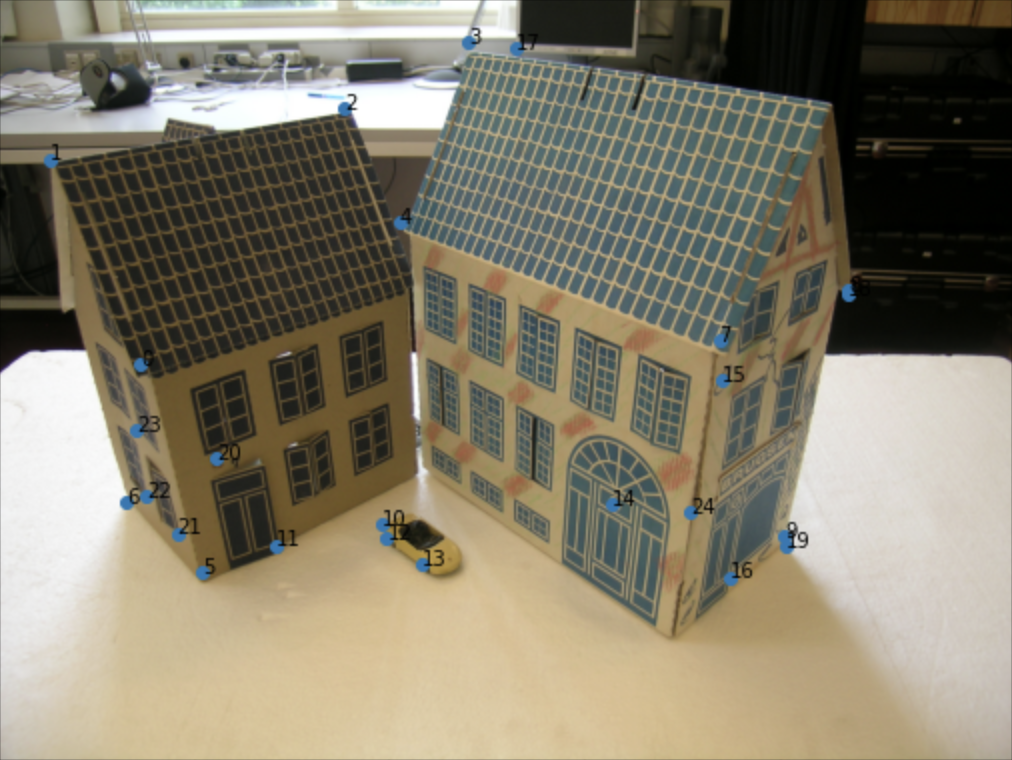
\includegraphics[width=\linewidth]{Materials/BaselineA}
	\end{subfigure}
	\hfill
	\begin{subfigure}{0.48\linewidth}
		\centering
		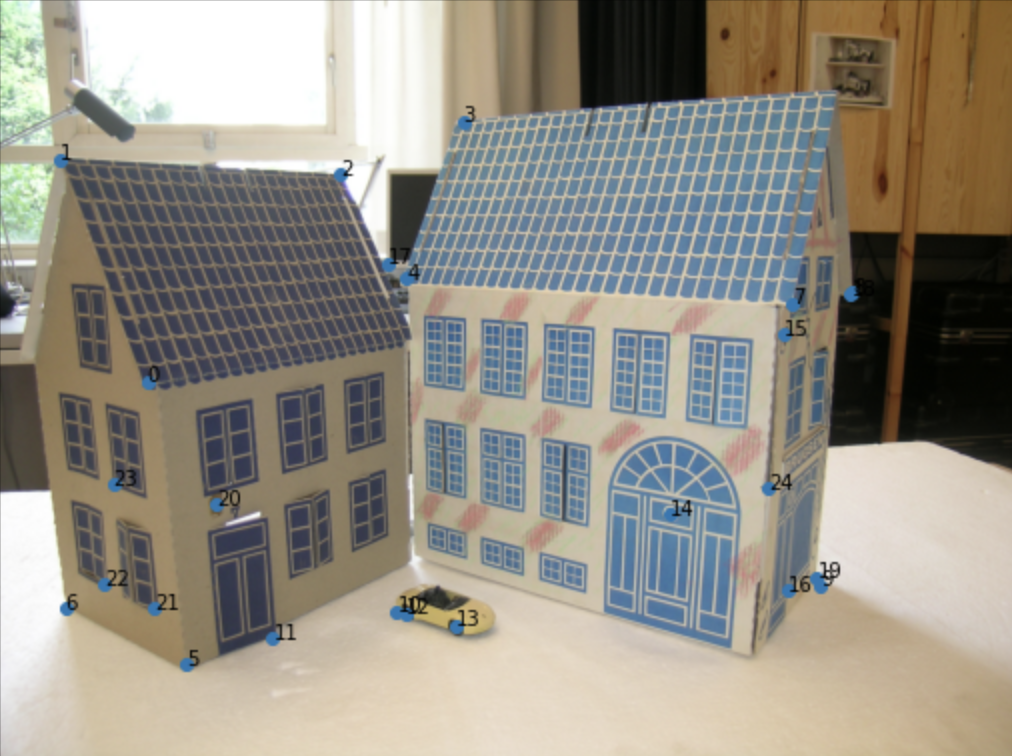
\includegraphics[width=\linewidth]{Materials/BaselineB}
	\end{subfigure}
	\caption{The 25 point correspondences between the two images found.}
	\label{correspondences}
\end{figure}
We will begin by establishing a baseline for comparison with the following experiments. This baseline will be the most naive / simple solution to estimating the fundamental matrix and bring the two images to scanline agreement. We begin by manually estimating 25 point correspondences between the two images which can be seen in \autoref{correspondences}. We now normalize the points found in each image separately by subtracting the mean of the points and dividing with their standard deviation. This gives us $T_A$ and $T_B$ which are transformation matrices for image A (left) and image B (right), and we will use these to denormalize the fundamental matrix. We can now estimate the fundamental matrix using the 8-point algorithm and after normalizing it by dividing through with index (3,3), we can report it to be:
\begin{equation*}
	F = \begin{bmatrix}
		-2.35e-06 & -1.81e-06 & -1.50e-02\\
		2.77e-06 & 2.43e-06 & -2.05e-02\\
		1.99e-02 &1.63e-02 & 1
	\end{bmatrix}
\end{equation*}
With the fundamental matrix we can now use \textit{opencv} and the function \textit{computeCorrespondEpilines} to determine the epipolar lines and draw them on the images by supplying the function with the points found in the images and the estimated fundamental matrix. This is done in \autoref{baselineepipolarlines}. Using opencv is simply for convenience to transform the points and estimating and drawing the epipolar lines.

\begin{figure}[h]
	\centering
	\begin{subfigure}{0.48\linewidth}
		\centering
		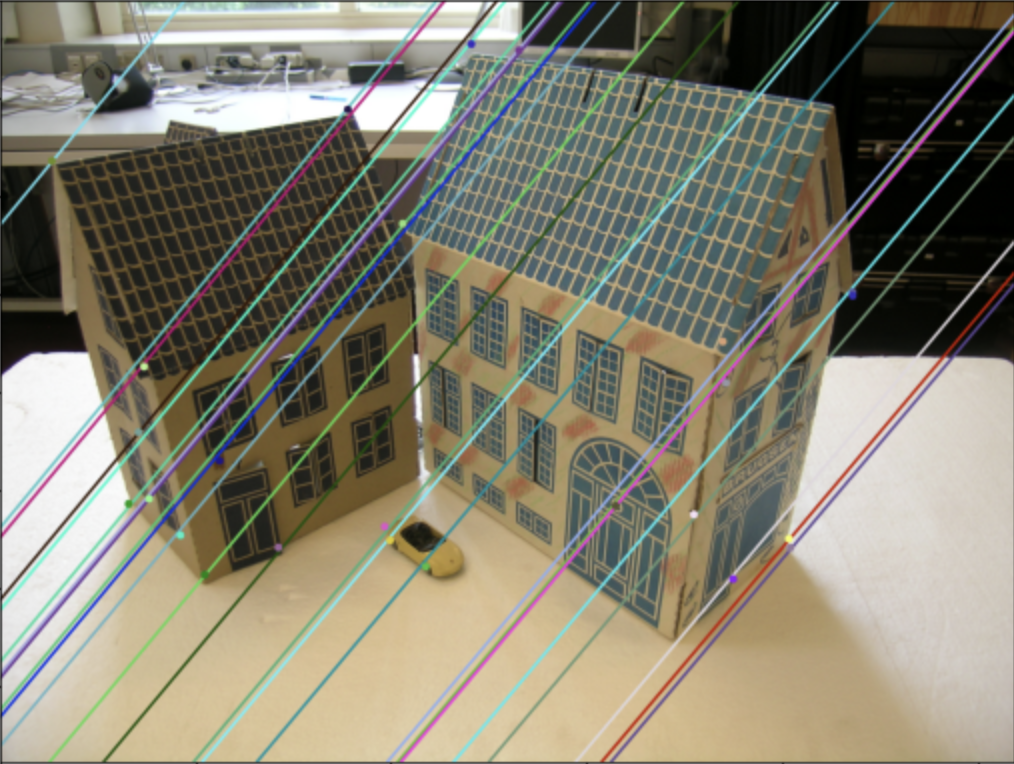
\includegraphics[width=\linewidth]{Materials/BaselineEpiA}
	\end{subfigure}
	\hfill
	\begin{subfigure}{0.48\linewidth}
		\centering
		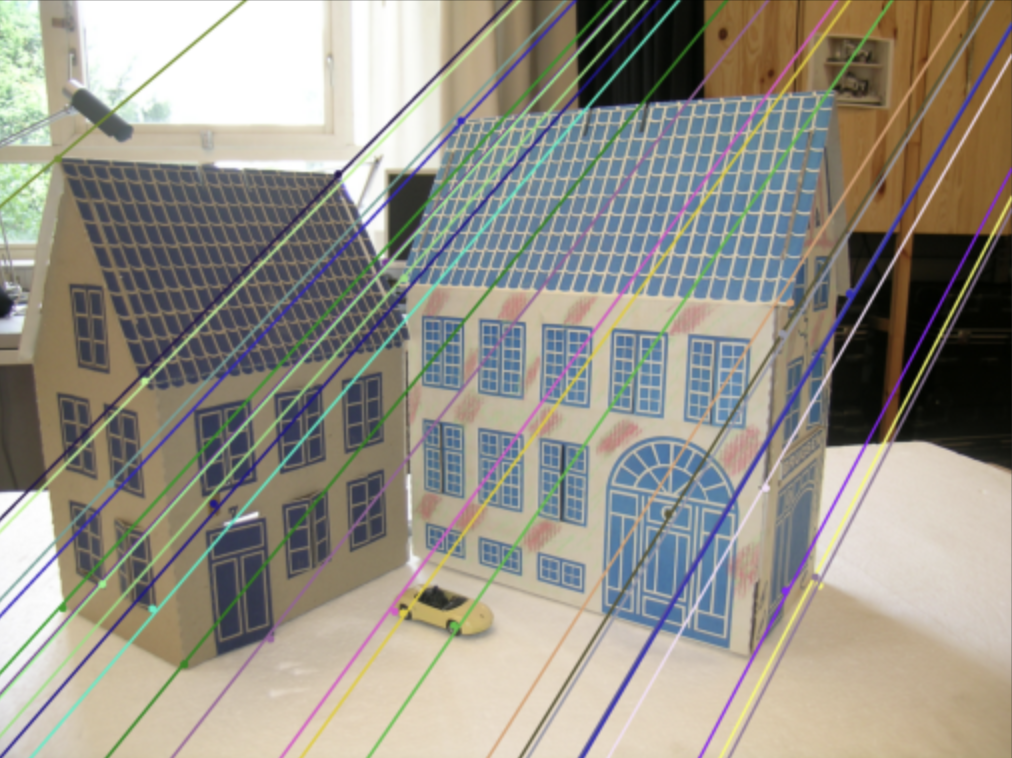
\includegraphics[width=\linewidth]{Materials/BaselineEpiB}
	\end{subfigure}
	\caption{Epipolar lines drawn on top of the two images.}
	\label{baselineepipolarlines}
\end{figure}
By computing the left and right null vectors of the fundamental matrix, $F$, we can get the coordinates of the epipoles. We find the left epipole, i.e. the optical center of the right camera projected into the left cameras view, to be at coordinates $[-104610.58, 127733.71]$, and the right epipole, i.e. the optical center of the left camera projected into the right cameras view, to be $[4577.86, -3312.85]$.\\
We can now bring the two images to scanline agreement using \textit{opencv} which can be seen in \autoref{baselineScanline}.
\begin{figure}[h]
	\centering
	\begin{subfigure}{0.48\linewidth}
		\centering
		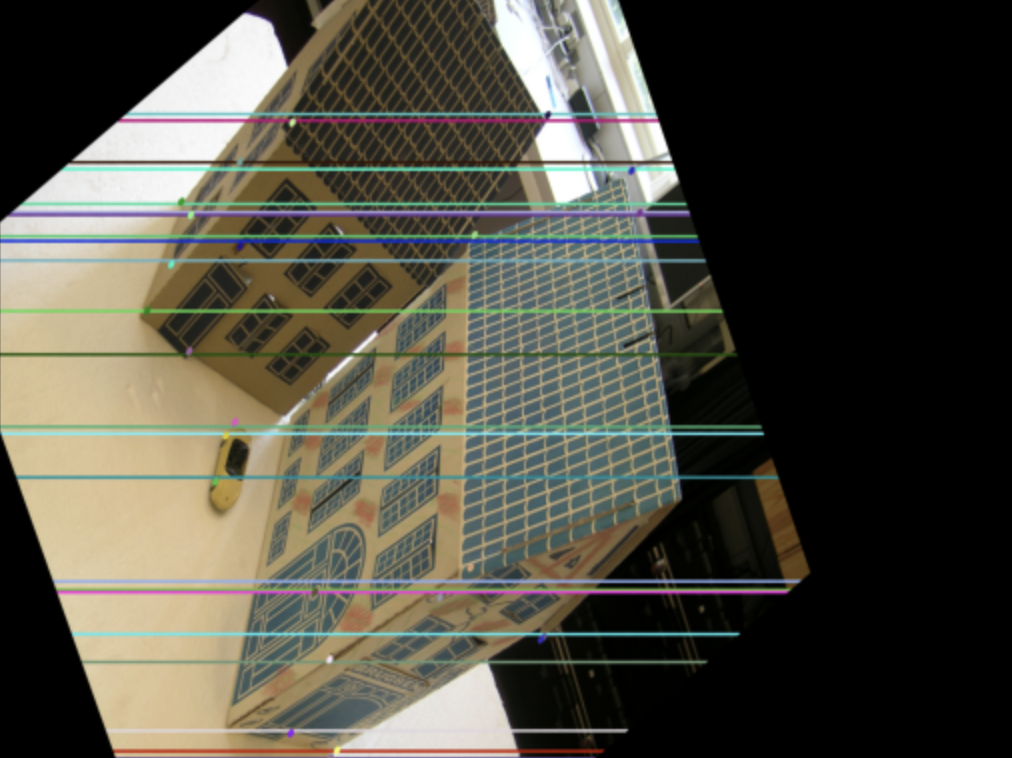
\includegraphics[width=\linewidth]{Materials/BaselineScanlineA}
	\end{subfigure}
	%\hfill
	\begin{subfigure}{0.48\linewidth}
		\centering
		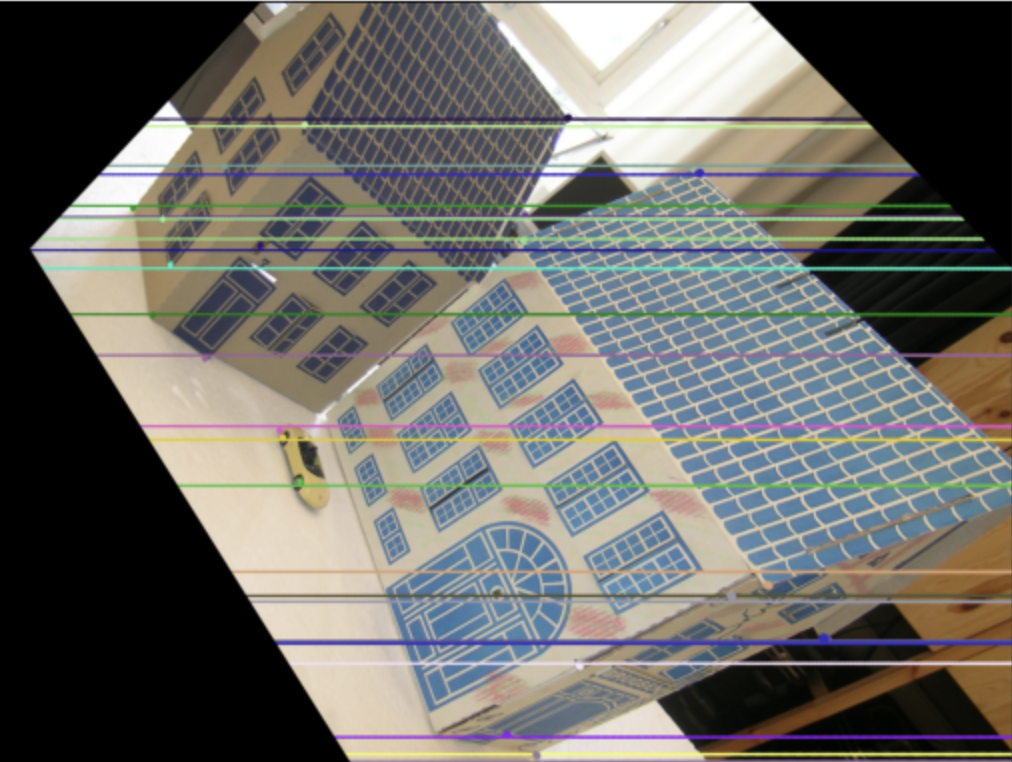
\includegraphics[width=\linewidth]{Materials/BaselineScanlineB}
	\end{subfigure}
	\caption{The baseline estimation brought to scanline agreement.}
	\label{baselineScanline}
\end{figure}
As the 'scanline agreement error' is ambiguous to me, I have chosen to follow the 'rectification error' from \cite{rectificationError} which measures the error by computing the mean and standard deviation of the \textit{y-disparity} (the vertical distance) between the points in image A and image B after rectification. Here we find a \textbf{mean} of \textbf{8.53} and a \textbf{standard deviation} of \textbf{7.41} which tells us our epipolar lines on average are fairly close to go through our points in the images, but the variance is also fairly high, which implies some of our points are very close, and some are quite far off.
\subsection{Ransac with baseline}
Ransac is a procedure which can be used to detect outlying data. We will use Ransac to sort out the correspondences we have found which are too imprecise to contribute to the estimation of the fundamental matrix. Using Ransac makes our estimation of the fundamental matrix more robust, and so we will also look at how robust our estimation becomes by adding random correspondences and then attempt to remove false correspondences with Ransac.

\subsubsection{Problems with Ransac}
Ransac can be implemented in a few different ways. One could simply use the largest inlier set found and return this. One could also estimate the error, and although a bigger inlier set might be found, it will only be accepted if the error is smaller than the previous best set (the set with the smallest error and largest number of inliers). Then, should the points used to compute the model be included when computing this error, or only points not used in the model estimation? In the latter we avoid bias, but the points used for model estimation will most likely be quantified as inliers. And perhaps most importantly, how does one estimate the thresholding used to determine inliers from outliers?\\
After some experimentation I have found using the largest inlier set gave the most consistent results and have thus chosen to use this implementation. For thresholding a constant threshold of 20 have been used. As the threshold is often simply chosen empirically, and the scanline agreement error from the baseline shows decent results, a threshold of 20 seems reasonable. The threshold could also have been estimated based on the standard deviation and a Chi distribution. To determine whether a correspondence is within this threshold, the \textit{Sampson distance} have been used as this seems to the most natural way to estimate the error, and it only involves the fundamental matrix.

\subsubsection{Error as function of falsely added correspondences}
We will now take a look at how robust the fundamental matrix estimation is when using Ransac. For this we take our 25 manually found correspondences and add a number of false correspondence before running Ransac. We then measure the mean and standard deviation of the scanline agreement error. As Ransac is a non-deterministic algorithm we might get rather different errors each run, and because we only are interested in the tendency of how the error behaves when adding false correspondences, we make 10 runs of Ransac and report the median mean and standard deviation found. This helps us avoid lucky or unlucky runs where the error reported is 'uncharacteristic' for the number of false correspondences added, and to avoid the skewness the average would give if one run reports something completely different than the other runs. The results can be seen in \autoref{BaselineRansacMedian}.

\begin{figure}[h]
	\centering
	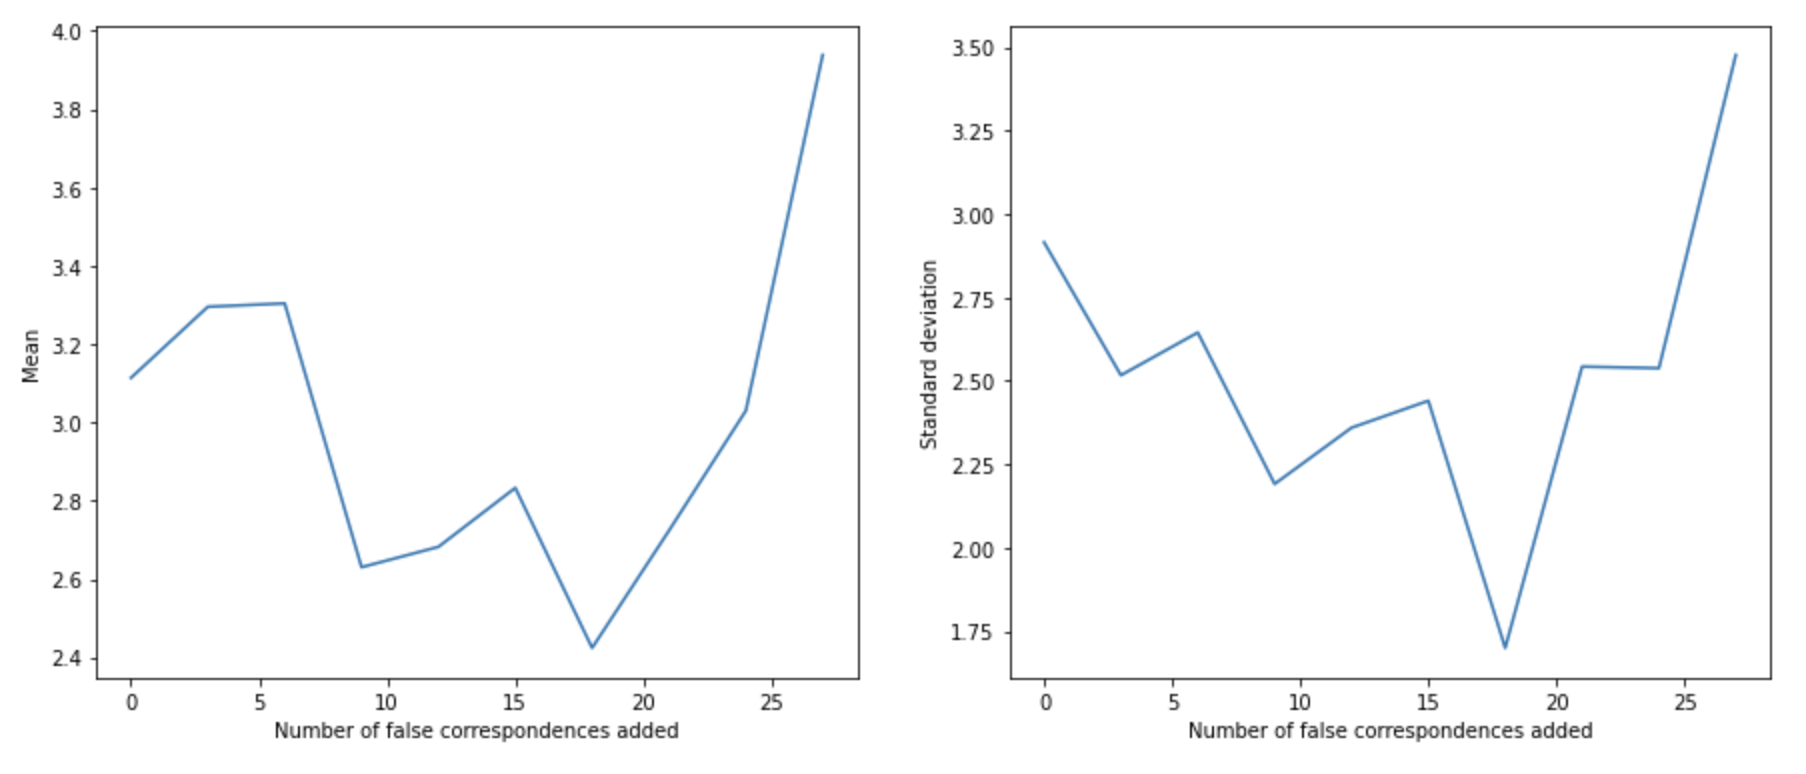
\includegraphics[width=\linewidth]{Materials/BaselineRansacMedian}
	\caption{The median mean and standard deviation after 10 Ransac runs with increasing number of false correspondences added to the manually found correspondences.}
	\label{BaselineRansacMedian}
\end{figure}
As seen the median mean and standard deviation only changes slightly, however, both show a tendency to grow quite rapidly when adding more than 18 false correspondences. This would equate to when the data consists of more than 42\% outliers Ransac begins to break down. This shows using Ransac makes the estimation of the fundamental matrix \textit{very} robust. We do however need to keep in mind that the false correspondences added here are random points in the two images, and so they with high probability fall \textit{completely} out of line with our inliers. This might be a reason why we can include so many false correspondences.

\subsubsection{Scanline agreement using Ransac}
Taking a visual look at using Ransac, we can report the result of running Ransac on the 25 correspondences manually found, and from the inliers, estimate the fundamental matrix. This can be seen in \autoref{BaselineRansac}.
\begin{figure}[h]
	\centering
	\begin{subfigure}{0.48\linewidth}
		\centering
		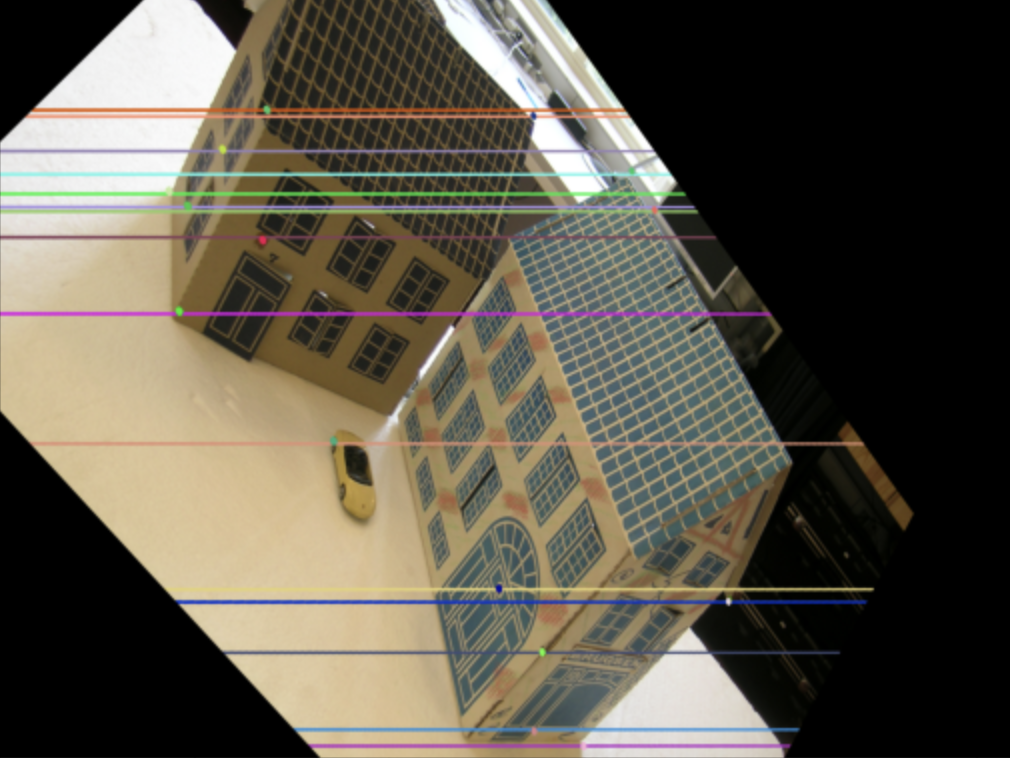
\includegraphics[width=\linewidth]{Materials/BaselineARansac}
	\end{subfigure}
	\begin{subfigure}{0.48\linewidth}
		\centering
		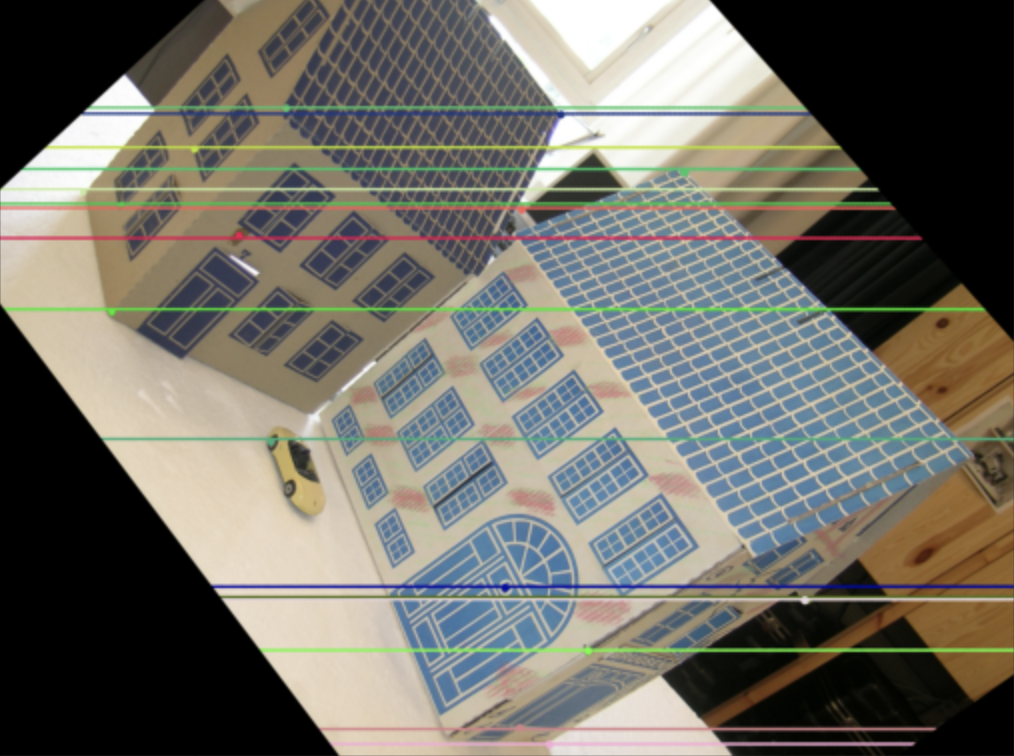
\includegraphics[width=\linewidth]{Materials/BaselineBRansac}
	\end{subfigure}
	\caption{Result of using Ransac on the original 25 correspondences before estimating the fundamental matrix and then bringing the images to scanline agreement.}
	\label{BaselineRansac}
\end{figure}
We here find a \textbf{mean} of \textbf{4.14} and a \textbf{standard deviation} of \textbf{2.57} of the scanline agreement error, which is a significant improvement over not using Ransac.
\subsection{Improved correspondences}
We will now improve our precision of our correspondences by applying the Harris corner detector. This has been done by extracting a small patch around our initial point location, and then run the Harris corner detector to find a more 'robust'/'easier to find again' location. Once these  points have then been found, we can estimate the fundamental matrix and scanline error to see if these improved points have an effect on the fundamental matrix estimation.

\subsubsection{Problems with Harris corner detection}
It is not obvious what the parameters for the Harris corner detector should be to give optimal results. Because a vast majority of the work in finding the improved points already was manual, I have tweaked the parameters for each original point until the Harris corner detector found a point which I would reckon would be easy to also find in the other image after applying the corner detector.\\
Another approach would have been to keep the parameters of the Harris corner detector constant and assume it is consistent. That is, if it does not find a perfect location, it will not find it in the other image either, but still find the same point in both image. In other words, if it makes a mistake, it make the same mistake in the other image. This would then have allowed us to discuss how well automatic detection could perform, whereas the first (and used) approach instead finds a 'lower bound' on the error we can get.

\subsubsection{Scanline agreement error}
If we simply estimate the fundamental with the improved correspondences we now find a \textbf{mean} of \textbf{1.92} and a \textbf{standard deviation} of \textbf{1.40} of the scanline agreement error. This is a fair bit better than running Ransac on the original correspondences, but as mentioned earlier, this is not representative for how an automatic detection would perform. We can now run Ransac on the improved correspondences and see the result in \autoref{ImprovedRansac}.

\begin{figure}[h]
	\centering
	\begin{subfigure}{0.48\linewidth}
		\centering
		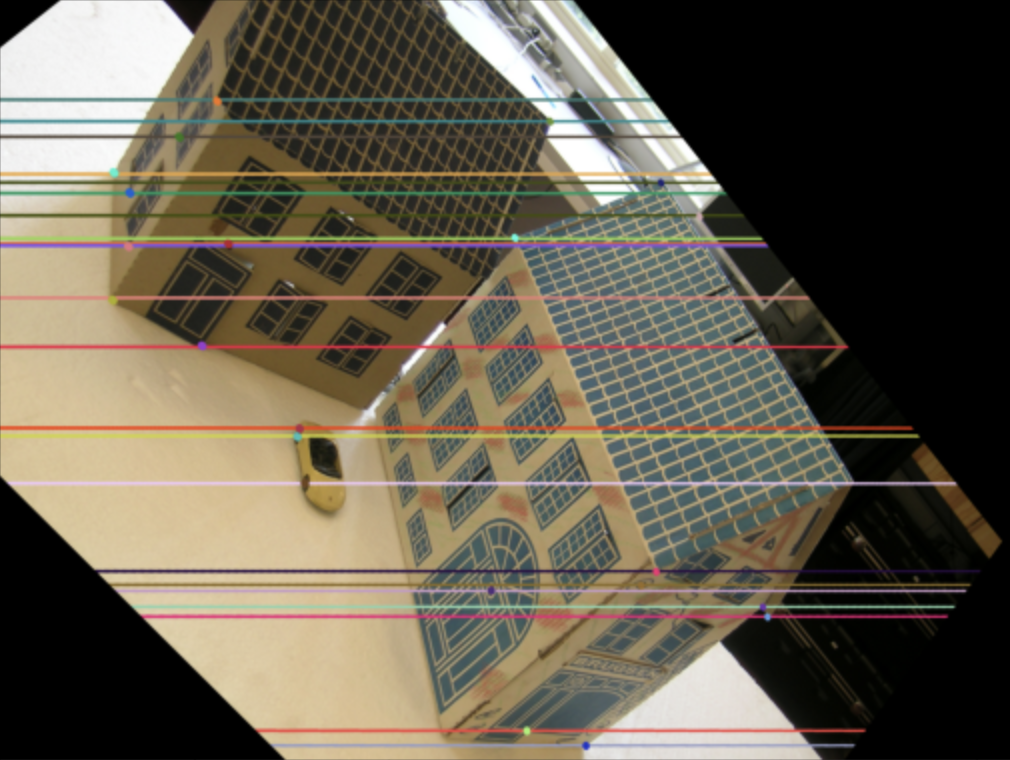
\includegraphics[width=\linewidth]{Materials/ImprovedARansac}
	\end{subfigure}
	\begin{subfigure}{0.48\linewidth}
		\centering
		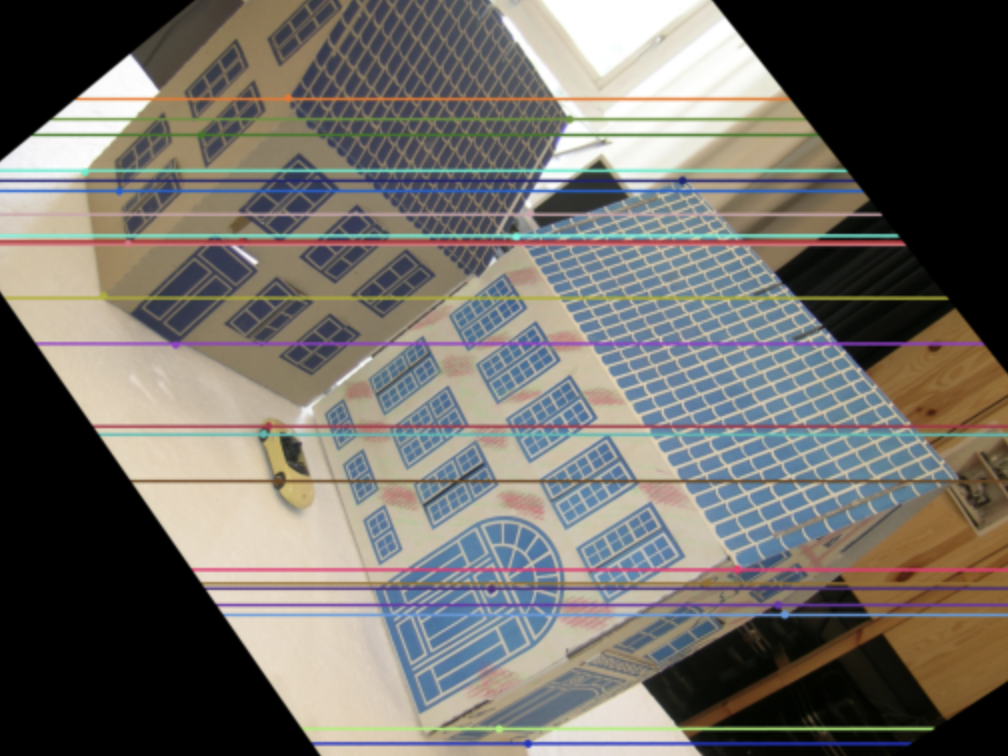
\includegraphics[width=\linewidth]{Materials/ImprovedBRansac}
	\end{subfigure}
	\caption{Result of using Ransac on the improved 25 correspondences before estimating the fundamental matrix and then bringing the images to scanline agreement.}
	\label{ImprovedRansac}
\end{figure}
We here find a \textbf{mean} of \textbf{1.52} and a \textbf{standard deviation} of \textbf{1.40} of the scanline agreement error, which is a slight improvement.

\subsubsection{Error as function of falsely added correspondences }
Looking at the error as a function of falsely added correspondences, now using the improved correspondences we get the results seen in \autoref{ImprovedRansacMedian}.

\begin{figure}[h]
	\centering
	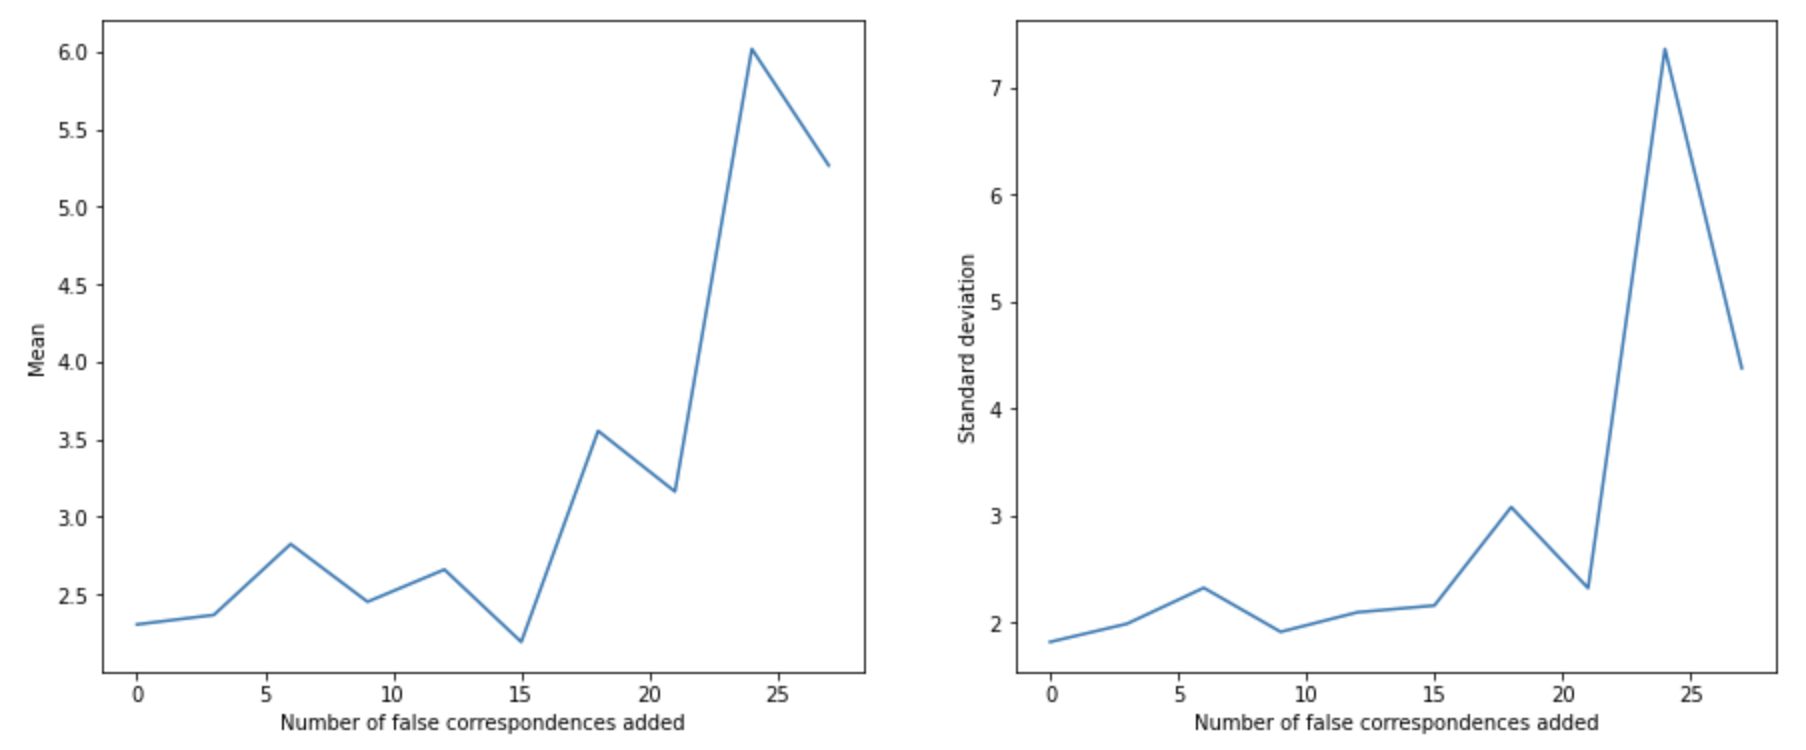
\includegraphics[width=\linewidth]{Materials/ImprovedRansacMedian}
	\caption{The median mean and standard deviation after 10 Ransac runs with increasing number of false correspondences added to the improved correspondences.}
	\label{ImprovedRansacMedian}
\end{figure}
We here see similar results as with the original correspondences, except a more clear tendency of increased error with increased number of false correspondences added. The more clear tendency might be a coincidence based on more similar Ransac runs or due to the run with 24 added false correspondences having a high error, and making it harder to see the small differences in mean and standard deviation. 
\subsection{Conclusion}
In conclusion we have seen SIFT and SURF detects roughly the same amount of features where ORB detects considerable less features. All three image descriptors perform somewhat bad when it comes to mean localization error, but this is likely due to aliasing or approximation error when transforming the images. When it comes to nearest neighbour mean average precision we see SIFT and ORB performs similar and fairly well, however SURF performs quite bad. This might be due to SIFT and ORB being both scale and rotation invariant, whereas SURF is only scale invariant. Lastly we have seen SIFT performs a lot better than both SURF and ORB when it comes to homography estimations, which is likely because SIFT both detects a lot of features and describes them well.\\
If we are to determine which of the three is better, it would depend on the task at hand. Although it is clear SIFT performs the best in the these experiments, it is also the slowest of the three. If the task requires fast feature matching it would not be possible to use SIFT, and we would need to trade performance for speed.

\begin{thebibliography}{9}
	\bibitem{rectificationError}
	Monnase, P., et. al. 'Three-step image rectification'.  British Machine Vision Conference.  Aug 2010.
\end{thebibliography}

\end{document}